\section{Description And Methodology}


\subsection{Initial Setup}
In this assignment the following peripherals need to be configured, buttons, LEDs, DAC, and some timer. The buttons are needed to allow interaction with the board. The buttons are configured to play different sounds when pushed. 




\subsection{Sound Wave Synthesis}
Sound is realised through sound waves which is created by oscillations. "An oscillator generates a consistent, repeating signals". These consistent signals can be used to create waves at various frequencies. Sound is actually the properties of the waves generated, with respect to frequency, amplitude, and period. The frequency determines the tone of the sound, the amplitude the strength, and the period the duration of the sound.  

There are various different approaches for generating these sound waves. The different waves have slightly different properties in regard to sound. To name a few different waves we have the sine wave, sawtooth wave, triangle wave and the square wave. These waves produces different sound characteristics {\bf more on this ? Sources and shit like that}. 

In case of this assignment, we have crated two different kind of waves, the square wave and the sawtooth wave. The square wave is created by calculating discrete samples based on the tone frequency and the oscillator frequency. Oscillator frequency divided by the tone frequency decides how often the values to the DAC should alternate, thereby producing an approximation of the note. The different notes supported by the program is as follows, A, B, C, D, E, and F. 


\begin{figure}[H]
  \centering
  % Trim er [left bottom right top]
  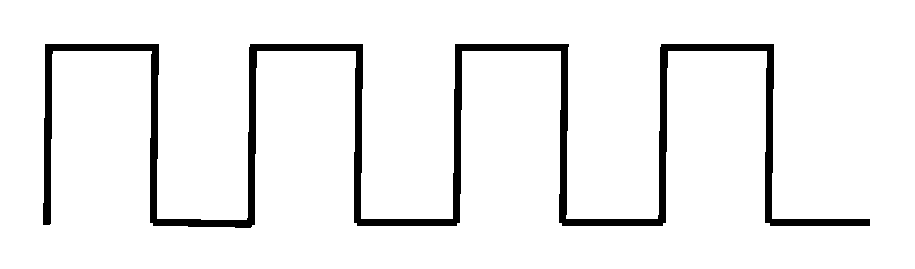
\includegraphics[clip, trim=0cm 0cm 0cm 0cm, width=4cm]{fig/square_wave.pdf}
  \caption{Square wave}
\end{figure}

\begin{figure}[H]
  \centering
  % Trim er [left bottom right top]
  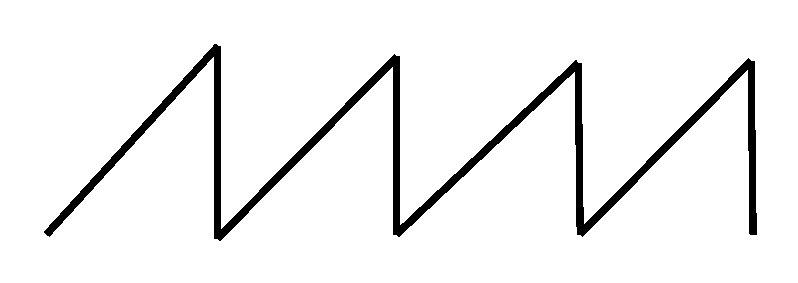
\includegraphics[clip, trim=0cm 0cm 0cm 0cm, width=4cm]{fig/sawtooth.pdf}
  \caption{Sawtooth wave}
\end{figure}



\subsection{Sound Sampling}
Sound can also be generated through pre computed samples. With this approach the sound waves are generated on some other platform. The samples produced are approximations to already existing sound waves. 


\subsection{Energy Optimization}
In order to decrease the energy consumption of our program we have taken various different methods to reduce the consumption. Instead of using the proposed timer\cite{compendium}, we are instead using the low energy timer, LETIMER0 \cite{EFM32GG-rm}. This timer runs at a lower frequency, but require an low frequency oscillator in order to be of any value. The advantage with this timer is that it uses less energy and is able to run in EM2.  



\subsection{User Control}











